\documentclass[12pt]{article}

\usepackage{sbc-template}

\usepackage{graphicx,url}
\usepackage{float}
\usepackage[brazil]{babel}   
%\usepackage[latin1]{inputenc}  
\usepackage[utf8]{inputenc}  
% UTF-8 encoding is recommended by ShareLaTex

     
\sloppy

\title{Simulador AtMega 328-p}

\author{Raul Ramires\inst{1}}


\address{Departamento de Informática -- Universidade Estadual de Maringá
  (UEM)\\
  Maringá -- PR -- Brazil
  \email{ra82293@uem.br}
}

\begin{document} 

\maketitle
     
\begin{resumo} 
O microcontrolador AtMega 328-p é amplamente usado em sistemas embarcados, como por exemplo o Arduino Uno. Esse microcontrolador permite realizar a leitura de vários tipos de sensores, controlar motores e outros dispositivos eletrônicos. A implementação de um ambiente de simulação permite ao usuário projetar circuitos e programações no microcontrolador sem a necessidade de possuir a unidade física.
\end{resumo}


\section{Introdução}

A implementação de um ambiente de simulação para o microcontrolador AtMega 328-p consiste em primeiramente implementar a execução do conjunto de instruções e as estruturas de registradores e memórias. As instruções do microcontrolador podem ser encontradas no manual \cite{man328p}.

\section{Arquitetura Atmega 328-p}
O microcontrolador Atmega 328-p possui 3 memórias diferentes, sendo elas:

\begin{itemize}
\item 32Kb de memória \textit{flash};
\item 2Kb de memória SRAM;
\item 1Kb de memória EEPROM.
\end{itemize}

Esse microcontrolador ainda possui 32 registradores de propósito geral de 8 bits, sendo que alguns trabalham em pares para permitir endereçamento de 16 bits. Registradores X, Y e Z atuam como ponteiros de 16 bits para o endereçamento do espaço de dados, o que permite um cálculo de endereços eficiente.

A Figura \ref{figBlocos} mostra o diagrama de blocos do microcontrolador.

\begin{figure}[H]
  \centering
  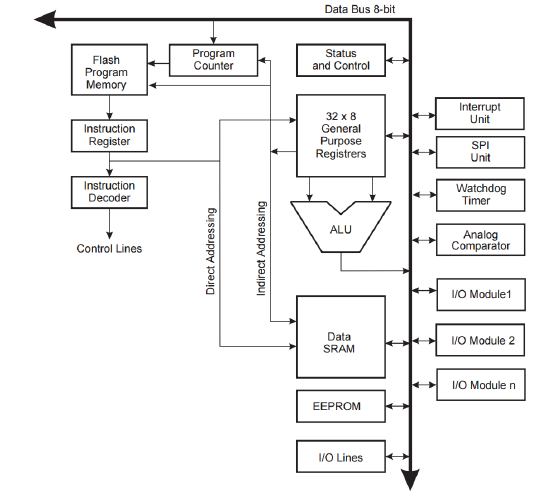
\includegraphics[scale=0.9]{Imagens/diagramaBlocos.png}
  \caption{Diagrama de blocos do microcontrolador.}
  \label{figBlocos}
\end{figure}

O registrador de estado (SREG) possui 8 bits e armazena algumas \textit{flags}, de acordo com a Figura \ref{figSREG}.

\begin{figure}[H]
  \centering
  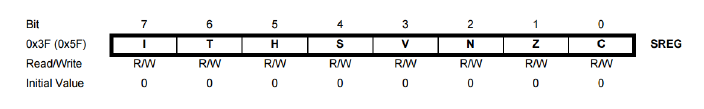
\includegraphics[scale=0.8]{Imagens/figSREG.png}
  \caption{Registrador de Estado SREG.}
  \label{figSREG}
\end{figure}

As \textit{flags} do registrador SREG são alteradas na execução de uma instrução, sendo que cada instrução altera \textit{flags} específicas de acordo com o manual. As \textit{flags} são as seguintes:

\begin{description}
\item[I] $\rightarrow$ Interrupção global;
\item[T] $\rightarrow$ Armazenamento de bit de cópia;
\item[H] $\rightarrow$ \textit{Half Carry};
\item[S] $\rightarrow$ Bit de sinal, $ S = N \oplus V$; 
\item[V] $\rightarrow$ \textit{Overflow} de complemento de 2;
\item[N] $\rightarrow$ Negativo;
\item[Z] $\rightarrow$ Zero;
\item[C] $\rightarrow$ \textit{Carry}. 
\end{description}

O microcontrolador possui um registrador PC (\textit{Program Counter}) de 14 bits que tem o propósito de apontar para a instrução que será executada. O valor de PC é incrementado a cada instrução executada, podendo ainda ser alterado por instruções de saltos.

\section{Implementação}
A implementação da execução do conjunto de instruções foi feita na linguagem C. Os registradores de propósito geral foram definidos como um \textit{array} de 32 posições do tipo \textit{uint\_8}. O registrador SREG foi implementado como uma \textit{struct} com os campos das \textit{flags} com o tipo de dado \textit{uint\_8}.

A Figura \ref{figRegisters} mostra a definição desses registradores no arquivo \textit{registers.h}.

\begin{figure}[H]
  \centering
  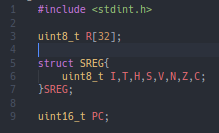
\includegraphics[scale=1]{Imagens/figRegisters.png}
  \caption{Definições dos registradores.}
  \label{figRegisters}
\end{figure}

Ainda não foram implementadas todas as instruções disponíveis no microcontrolador, mas estão implementadas uma grande parte das instruções. As instruções estão programadas nos arquivos \textit{instruction\_set.c} e \textit{instruction\_set.h}.

\subsection{Instruções Aritméticas}
Foram implementadas as instruções aritméticas de soma com e sem \textit{carry}. A Figura \ref{figADD} mostra o código da instrução de soma sem \textit{carry}.

\begin{figure}[H]
  \centering
  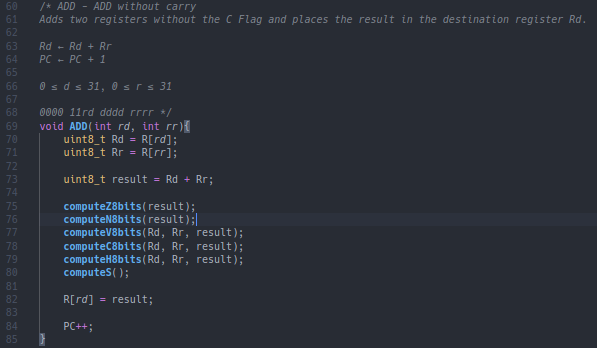
\includegraphics[scale=0.8]{Imagens/figADD.png}
  \caption{Instrução de soma sem \textit{carry}.}
  \label{figADD}
\end{figure}

As funções auxiliares para cálculo das \textit{flags} do registrador de estado SREG estão implementadas nos arquivos \textit{functions.c} e \textit{functions.h}.

\subsection{Instruções Lógicas}
Foram implementadas a maior parte das instruções lógicas, como por exemplo a operação \textit{AND} entre dois registradores, alterando as devidas \textit{flags} do registrador de estado. A Figura \ref{figAND} mostra o código da operação \textit{AND} entre dois registradores.

\begin{figure}[H]
  \centering
  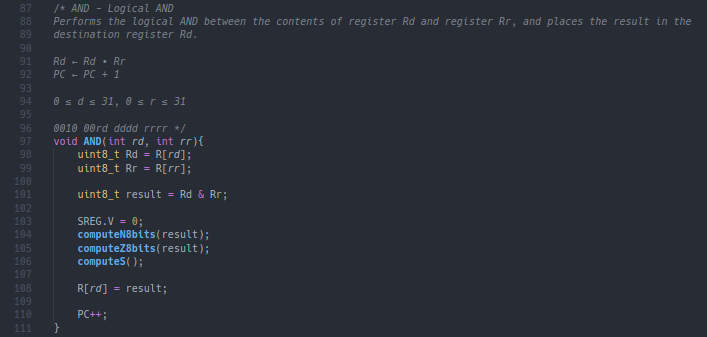
\includegraphics[scale=0.8]{Imagens/figAND.png}
  \caption{Instrução \textit{AND} entre dois registradores.}
  \label{figAND}
\end{figure}

\subsection{Instruções de Saltos}
Foram implementadas todas as funções de saltos disponíveis no conjunto de instruções do microcontrolador. Essas funções consistem apenas em alterar o valor do registrador PC (\textit{Program Counter}) de acordo com uma dada condição.

\section{Próximos Passos}
Para incrementar a implementação do ambiente de simulação são sugeridos os seguintes passos:

\begin{itemize}
\item Implementação das instruções que estão faltando;
\item Implementação dos registradores que controlam as portas digitais do microcontrolador (\textit{PORTD, PORTB});
\item Implementação dos registradores que controlam a direção dos dados dos pinos como entrada ou saída (\textit{DDRD, DDRB});
\item Implementação da memória onde será armazenado o código das instruções que serão executadas.
\end{itemize}

\bibliographystyle{sbc}
\bibliography{sbc-template}

\end{document}
